%!TEX root = ./main.tex

%\begin{figure*}[t]
%\centering
    %\begin{subfigure}[t]{0.45\textwidth}
    %\includegraphics[width=0.9\columnwidth]{Olivette}
    %\end{subfigure}
    %~
    %\begin{subfigure}[t]{0.45\textwidth}
    %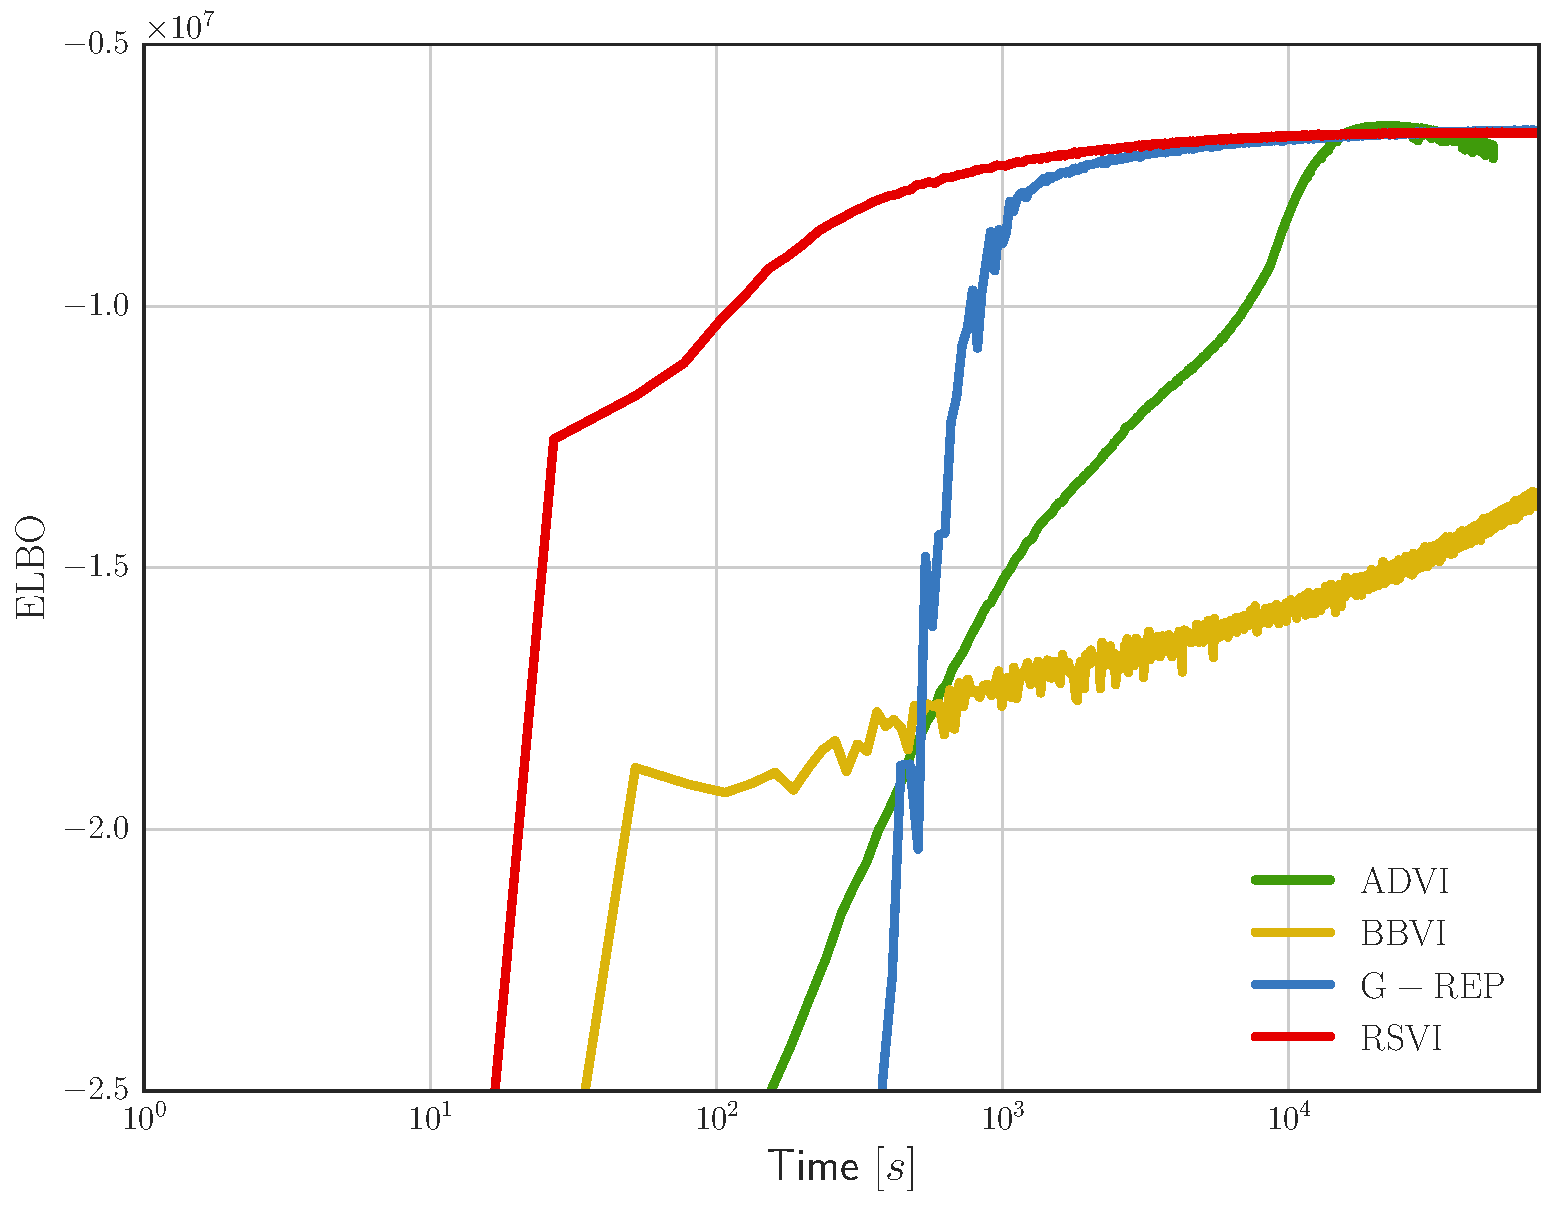
\includegraphics[width=0.9\columnwidth]{Olivette_time}
    %\end{subfigure}
    %\caption{\gls{ELBO} for the sparse gamma \gls{DEF}, applied to the Olivetti faces dataset, for \gls{ADVI}, \gls{BBVI}, \gls{G-REP}, and \gls{RS-VI}. \emph{Left:} As a function of iterations between comparable methods. \emph{Right:} As a function of wall-clock-time for all methods.}\label{fig:olivetteDEF}
%\end{figure*}

\section{Experiments}\label{sec:experiments}
\glsresetall

In Section~\ref{sec:examples} we compared \gls{RS-VI} with \gls{G-REP} and found a substantial variance reduction on synthetic examples. Here we evaluate \gls{RS-VI} on a more challenging model, the sparse gamma \gls{DEF}~\citep{Ranganath2015}. On two real datasets, we compare \gls{RS-VI} with state-of-the-art methods: \gls{ADVI} \citep{Kucukelbir2015,Kucukelbir2016}, \gls{BBVI} \citep{Ranganath2014}, and \gls{G-REP} \citep{RuizTB2016}.

\parhead{Data.}
The datasets we consider are the Olivetti faces\footnote{\url{http://www.cl.cam.ac.uk/research/dtg/attarchive/facedatabase.html}} and \gls{NIPS} 2011 conference papers. The Olivetti faces dataset consists of $64\times 64$ gray-scale images of human faces in $8$ bits, \ie, the data is discrete and in the set $\{0,\ldots,255\}$. In the \gls{NIPS} dataset we have documents in a bag-of-words format with an effective vocabulary of $5715$ words. 
%To be able to compare our method with that of \citet{RuizTB2016} we choose $3$ layers, respectively with $100$, $40$, and $15$ components in each. 
\begin{figure}[t]
\centering
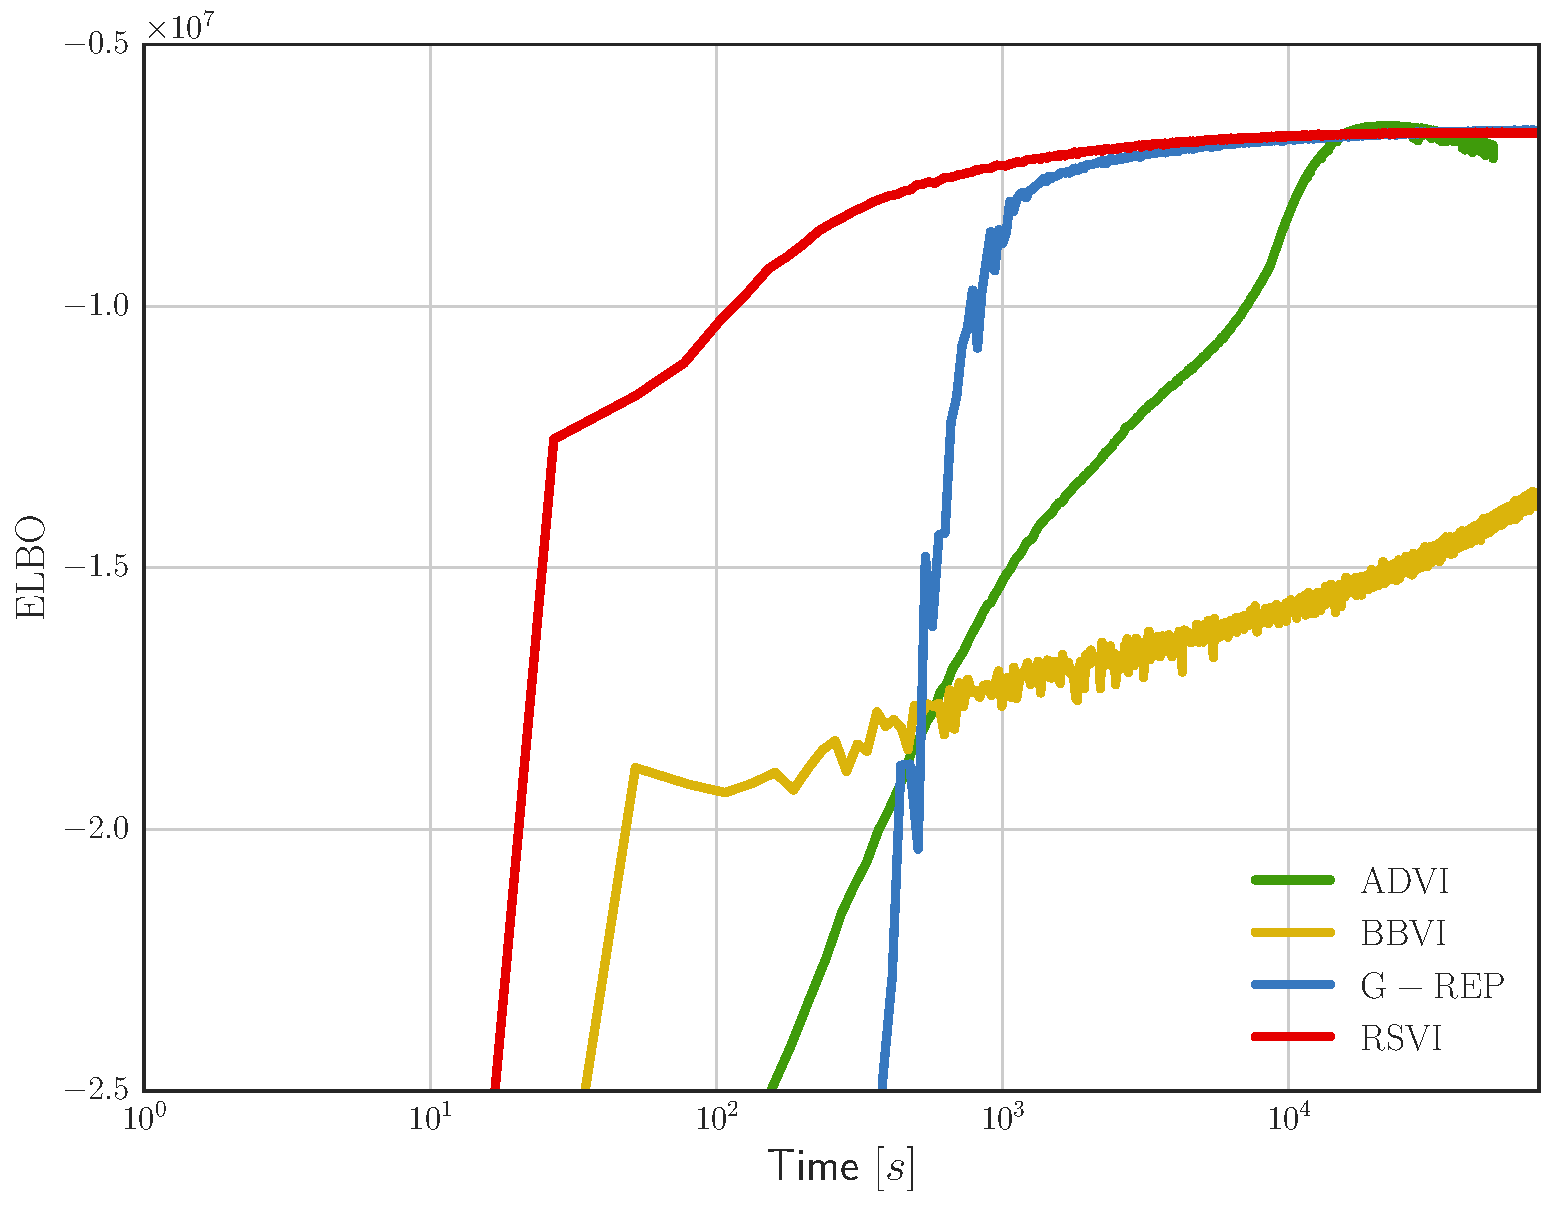
\includegraphics[width=0.9\columnwidth]{Olivette_time}
\caption{\gls{RS-VI} (this paper) presents a significantly faster initial improvement of the \gls{ELBO} as a function of wall-clock time. The model is a sparse gamma \gls{DEF}, applied to the Olivetti faces dataset, and we compare with \gls{ADVI} \citep{Kucukelbir2016}, \gls{BBVI} \citep{Ranganath2014}, and \gls{G-REP} \citep{RuizTB2016}. }\label{fig:olivetteDEF}
\end{figure}

\begin{table*}[t]
\centering
\begin{subtable}{0.45\textwidth}
\begin{tabular}{cccc}
\toprule
 & \gls{RS-VI} $B=1$ & \gls{RS-VI} $B=4$ &\gls{G-REP}\\ \hline
Min & $6.0\mathrm{e}{-4}$ & $1.2\mathrm{e}{-3}$ & $2.7\mathrm{e}{-3}$\\
Median & $\mathbf{9.0\mathrm{e}{7}}$ & $\mathbf{2.9\mathrm{e}{7}}$ & $1.6\mathrm{e}{12}$\\
Max & $1.2\mathrm{e}{17}$ & $\mathbf{3.4\mathrm{e}{14}}$ & $1.5\mathrm{e}{17}$ \\ \bottomrule 
\end{tabular}
%\caption{Estimated variance, based on $10$ samples, of the \gls{G-REP} and \gls{RS-VI} (for $B=1,4$) gradients for the initialization point. Estimated for the NIPS dataset.}\label{tab:vardef1}
\end{subtable}
\hspace*{15pt}
\begin{subtable}{0.45\textwidth}
\begin{tabular}{cccc}
\toprule
 & \gls{RS-VI} $B=1$ & \gls{RS-VI} $B=4$ &\gls{G-REP}\\ \hline
Min & $1.8\mathrm{e}{-3}$ & $1.5\mathrm{e}{-3}$ & $2.6\mathrm{e}{-3}$\\
Median & $1.2\mathrm{e}{4}$ & $\mathbf{4.5\mathrm{e}{3}}$ & $1.5\mathrm{e}{7}$\\
Max & $1.4\mathrm{e}{12}$ & $\mathbf{1.6\mathrm{e}{11}}$ & $3.5\mathrm{e}{12}$ \\ \bottomrule
\end{tabular}
%\caption{Estimated variance, based on $10$ samples, of the \gls{G-REP} and \gls{RS-VI} (for $B=1,4$) gradients for parameters at step $2600$ in \gls{RS-VI}. Estimated for the NIPS dataset.}\label{tab:vardef2}
\end{subtable}
\caption{The \gls{RS-VI} gradient (this paper) exhibits lower variance than \gls{G-REP} \citep{RuizTB2016}. We show estimated variance, based on $10$ samples, of \gls{G-REP} and \gls{RS-VI} (for $B=1,4$ shape augmentation steps), for parameters at the initialization point (\emph{left}) and at iteration $2600$ in \gls{RS-VI} (\emph{right}), estimated for the \gls{NIPS} data.}\label{tab:vardef}
\end{table*}


\parhead{Model.}
The sparse gamma \gls{DEF} \citep{Ranganath2015} is a multi-layered probabilistic model that mimics the architecture of deep neural networks. It models the data using a set of local latent variables $z_{n,k}^\ell$ where $n$ indexes observations, $k$ components, and $\ell$ layers. These local variables are connected between layers through global weights $w_{k,k'}^\ell$. The observations are $x_{n,d}$, where $d$ denotes dimension. The joint probabilistic model is defined as
\begin{align}
\begin{split}
z_{n,k}^\ell &\sim \gam\left(\alpha_z,\frac{\alpha_z}{\sum_{k'} w_{k,k'}^\ell z_{n,k'}^{\ell+1}} \right), \\
x_{n,d} &\sim \mathrm{Poisson}\left(\sum_{k} w_{k,d}^0 z_{n,k}^1 \right).
\end{split}
\end{align}
We set $\alpha_z=0.1$ in the experiments. All priors on the weights are set to $\gam(0.1,0.3)$, and the top-layer local variables priors are set to $\gam(0.1,0.1)$. We use $3$ layers, with $100$, $40$, and $15$ components in each. 
This is the same model that was studied by \citet{RuizTB2016}, where \gls{G-REP} was shown to outperform both \gls{BBVI} (with control variates and Rao-Blackwellization), as well as \gls{ADVI}. In the experiments we follow their approach and parameterize the variational approximating gamma distribution using the shape and mean. To avoid constrained optimization we use the transform $\theta = \log(1+\exp(\vartheta))$ for non-negative variational parameters $\theta$, and optimize $\vartheta$ in the unconstrained space.


\parhead{Results.}
For the Olivetti faces we explore ${\eta\in\{0.75,1,2,5\}}$ and show the resulting \gls{ELBO} of the best one in Figure~\ref{fig:olivetteDEF}. We can see that \gls{RS-VI} has a significantly faster initial improvement than any of the other methods.\footnote{%
	The results of \gls{G-REP}, \gls{ADVI} and \gls{BBVI} where reproduced with permission from \citet{RuizTB2016}.%
} 
%The wall-clock time for \gls{RS-VI} is based on a Python implementation (average $1.5$s per iteration) using the automatic differentiation package autograd \citep{autograd}. The others have been implemented in MatLab with hand-derived derivatives and thus the running times are not directly comparable. In fact, we also implemented \gls{G-REP} in Python and found \gls{RS-VI} to be approximately two times faster. One reason for this is that the transformations based on rejection sampling are cheaper to evaluate. Indeed, the research literature on rejection sampling is heavily focused on finding cheap and efficient transformations.
%\fr{The paragraph above is too confusing. Let's re-do the plot, and scale the time of RS-VI (or, the time of the other methods) accordingly so that they are "approximately comparable". I propose to use this paragraph instead:} 
The wall-clock time for \gls{RS-VI} is based on a Python implementation (average $1.5$s per iteration) using the automatic differentiation package autograd \citep{autograd}. We found that \gls{RS-VI} is approximately two times faster than \gls{G-REP} for comparable implementations. One reason for this is that the transformations based on rejection sampling are cheaper to evaluate. Indeed, the research literature on rejection sampling is heavily focused on finding cheap and efficient transformations.

%\cn{Mainly real data-example with the sparse gamma DEF, see Figure~\ref{fig:olivetteDEF} for preliminary results}

For the \gls{NIPS} dataset, we now compare the variance of the gradients between the two estimators, \gls{RS-VI} and \gls{G-REP}, for different shape augmentation steps $B$. In Table~\ref{tab:vardef} we show the minimum, median, and maximum values of the variance across all dimensions. We can see that \gls{RS-VI} again clearly outperforms \gls{G-REP} in terms of variance. Moreover, increasing the number of augmentation steps $B$ provides even further improvements.% We have also studied the variance without shape augmentation and \gls{RS-VI} tends to give a significant variance reduction in this case too. However when we force all shapes $\alpha \geq 1$, %\fr{include in table?}

%\begin{table}[t]
%\centering
%\begin{tabular}{cccc}
 %& \gls{RS-VI} $B=1$ & \gls{RS-VI} $B=4$ &\gls{G-REP}\\
%\hline
%Min & $1.8\mathrm{e}{-3}$ & $1.5\mathrm{e}{-3}$ & $2.6\mathrm{e}{-3}$\\
%Median & $1.2\mathrm{e}{4}$ & $\mathbf{4.5\mathrm{e}{3}}$ & $1.5\mathrm{e}{7}$\\
%Max & $1.4\mathrm{e}{12}$ & $\mathbf{1.6\mathrm{e}{11}}$ & $3.5\mathrm{e}{12}$
%\end{tabular}
%\caption{Estimated variance, based on $10$ samples, of the \gls{G-REP} and \gls{RS-VI} (for $B=1,4$) gradients for parameters at step $2600$ in \gls{RS-VI}. Estimated for the NIPS dataset.}\label{tab:vardef2}
%\end{table}

